% !TEX root = ../main.tex
\subsection{Acceptance Correction Results}
\label{14.20::acceptance_correction_results}
% TODO. acceptance correction effect on acceptance.

% --+ Acceptance correction results +-------------------------------------------
    % The plots to the right of Figure \ref{fig::acc_corr} show the number of generated events in red and the number of simulated events that were successfully reconstructed out of that set in blue.
    % Each one is presented in integrated kinematical region for the other variables.
    % As described before, the acceptance correction factor comes from the quotient of the number of simulated events, $N_\text{simul}$ versus the number of thrown events, $N_\text{thrown}$.

% --+ Plots +-------------------------------------------------------------------
    % \begin{figure}[hbtp]
    %     % Q2.
    %     \begin{subfigure}{.5\textwidth}
    %         \centering
    %         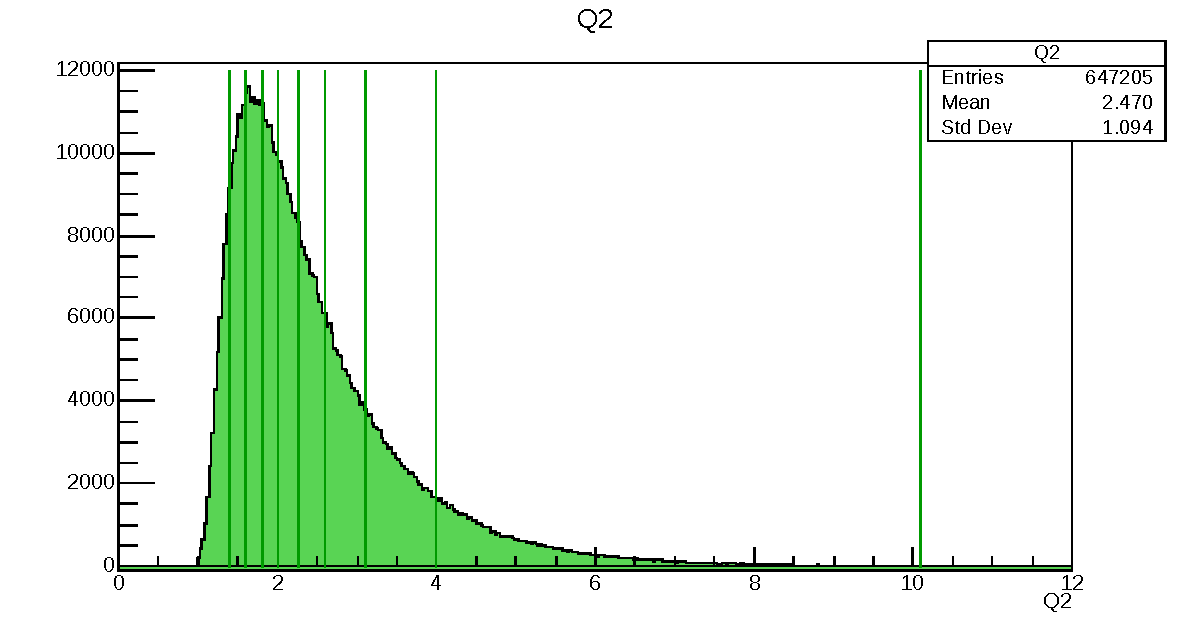
\includegraphics[width=\linewidth]{13dataanalysis/img/40_accbins_q2.pdf}
    %         % \caption{$Q^2$ bins.}
    %         \label{fig::acc_corr_bins_q2}
    %     \end{subfigure}
    %     \begin{subfigure}{.5\textwidth}
    %         \centering
    %         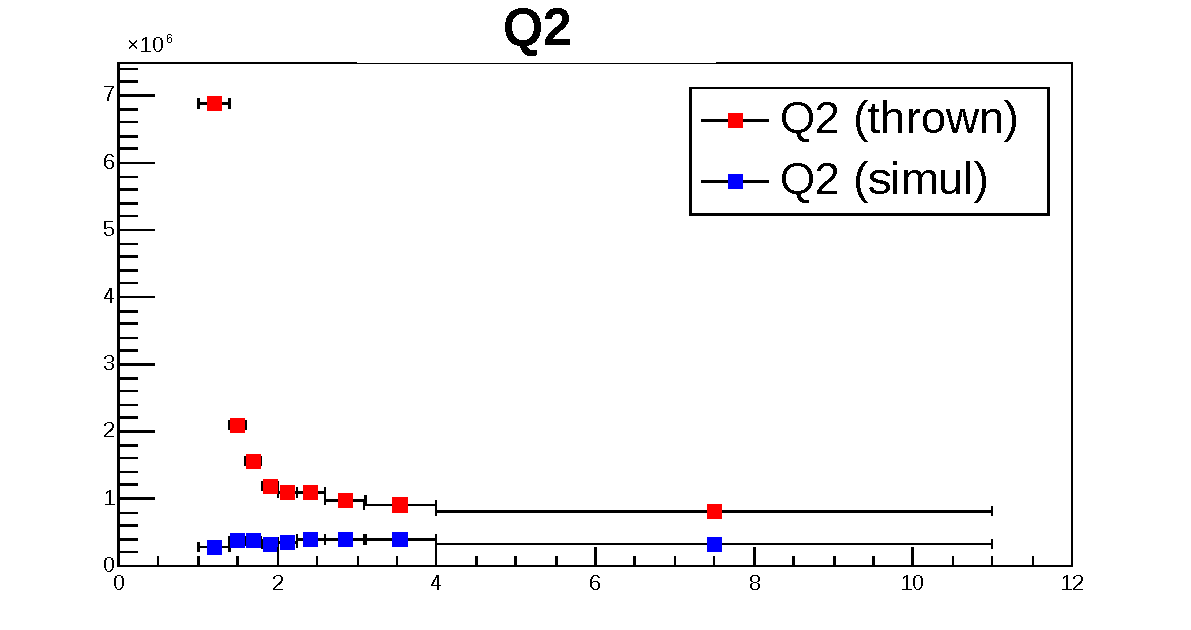
\includegraphics[width=\linewidth]{13dataanalysis/img/40_acccorr_q2.pdf}
    %         % \caption{$Q^2$ acceptance correction results.}
    %         \label{fig::acc_corr_q2}
    %     \end{subfigure}
    %
    %     % nu.
    %     \begin{subfigure}{.5\textwidth}
    %         \centering
    %         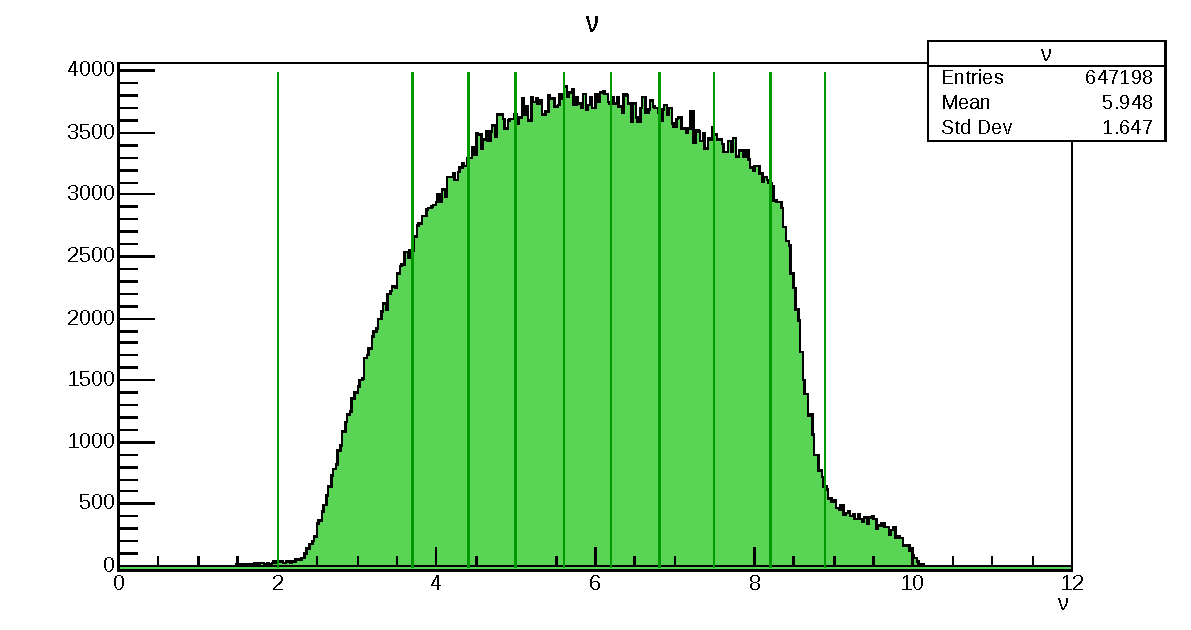
\includegraphics[width=\linewidth]{13dataanalysis/img/40_accbins_nu.pdf}
    %         % \caption{$\nu$ bins.}
    %         \label{fig::acc_corr_bins_nu}
    %     \end{subfigure}
    %     \begin{subfigure}{.5\textwidth}
    %         \centering
    %         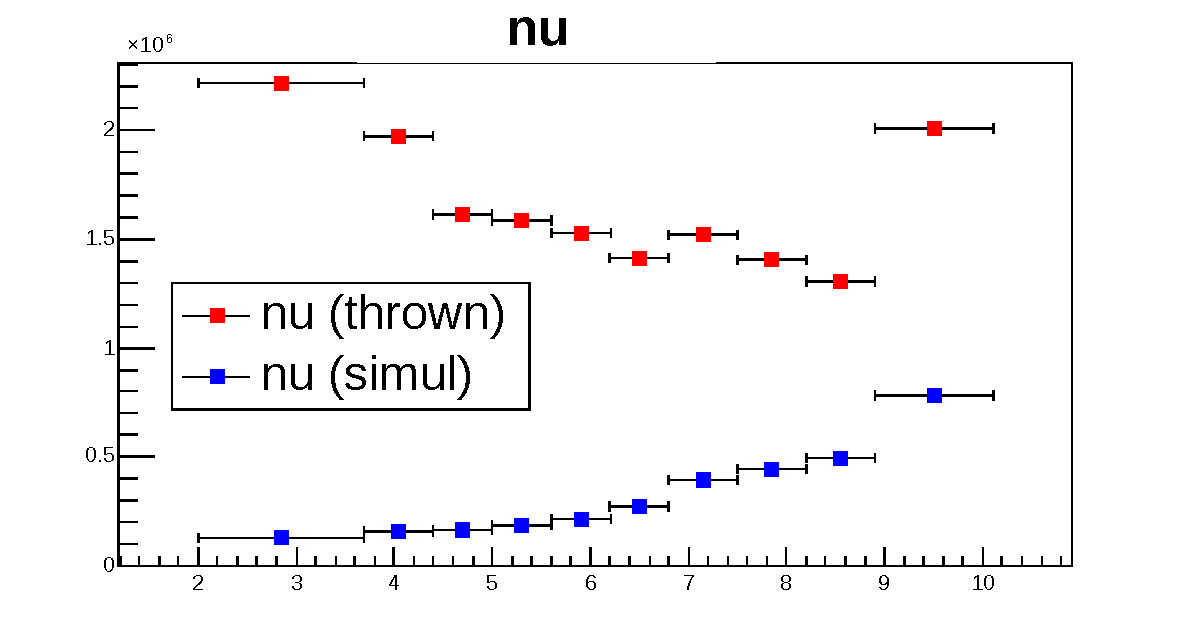
\includegraphics[width=\linewidth]{13dataanalysis/img/40_acccorr_nu.pdf}
    %         % \caption{$\nu$ acceptance correction results.}
    %         \label{fig::acc_corr_nu}
    %     \end{subfigure}
    %
    %     % zh.
    %     \begin{subfigure}{.5\textwidth}
    %         \centering
    %         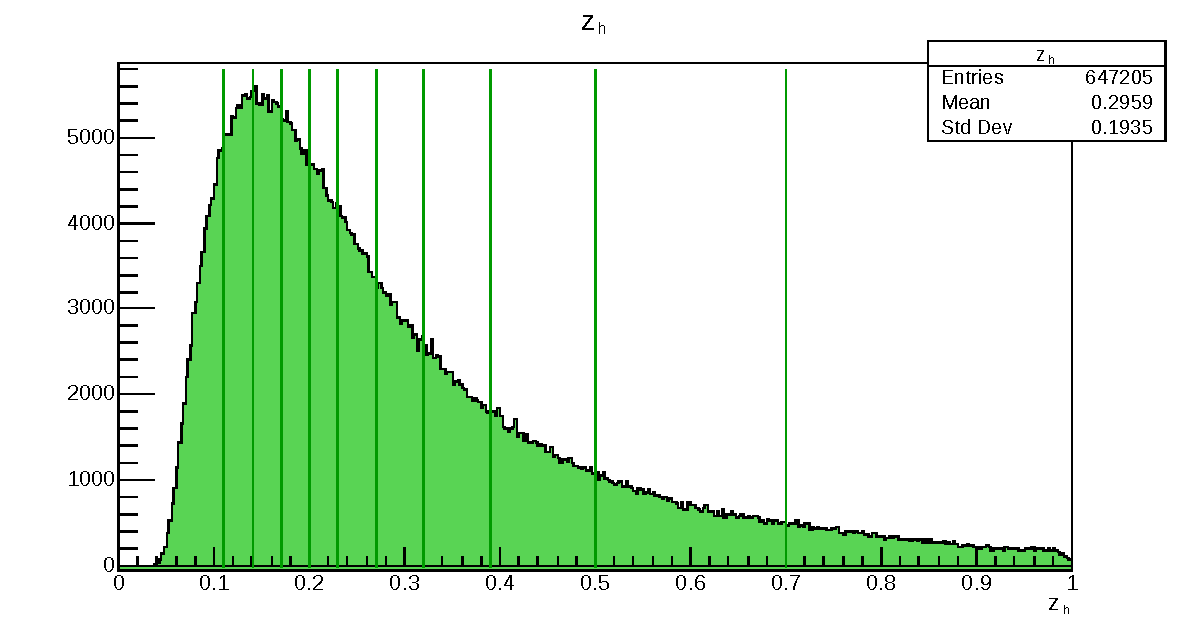
\includegraphics[width=\linewidth]{13dataanalysis/img/40_accbins_zh.pdf}
    %         % \caption{$z_h$ bins.}
    %         \label{fig::acc_corr_bins_zh}
    %     \end{subfigure}
    %     \begin{subfigure}{.5\textwidth}
    %         \centering
    %         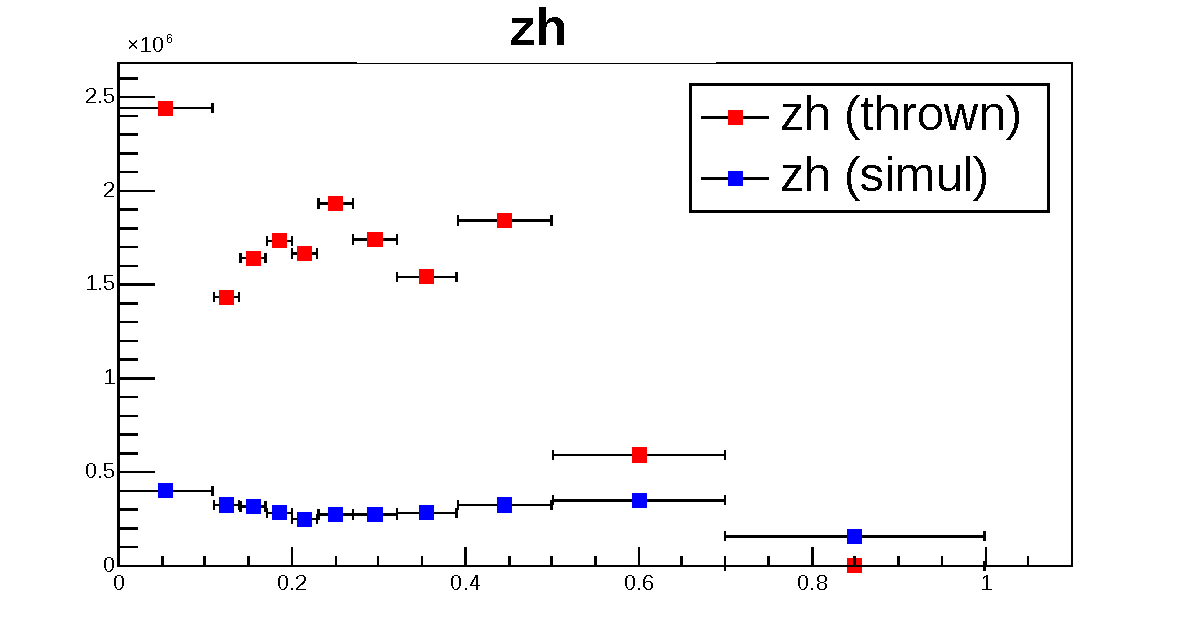
\includegraphics[width=\linewidth]{13dataanalysis/img/40_acccorr_zh.pdf}
    %         % \caption{$z_h$ acceptance correction results.}
    %         \label{fig::acc_corr_zh}
    %     \end{subfigure}
    %
    %     % PT2.
    %     \begin{subfigure}{.5\textwidth}
    %         \centering
    %         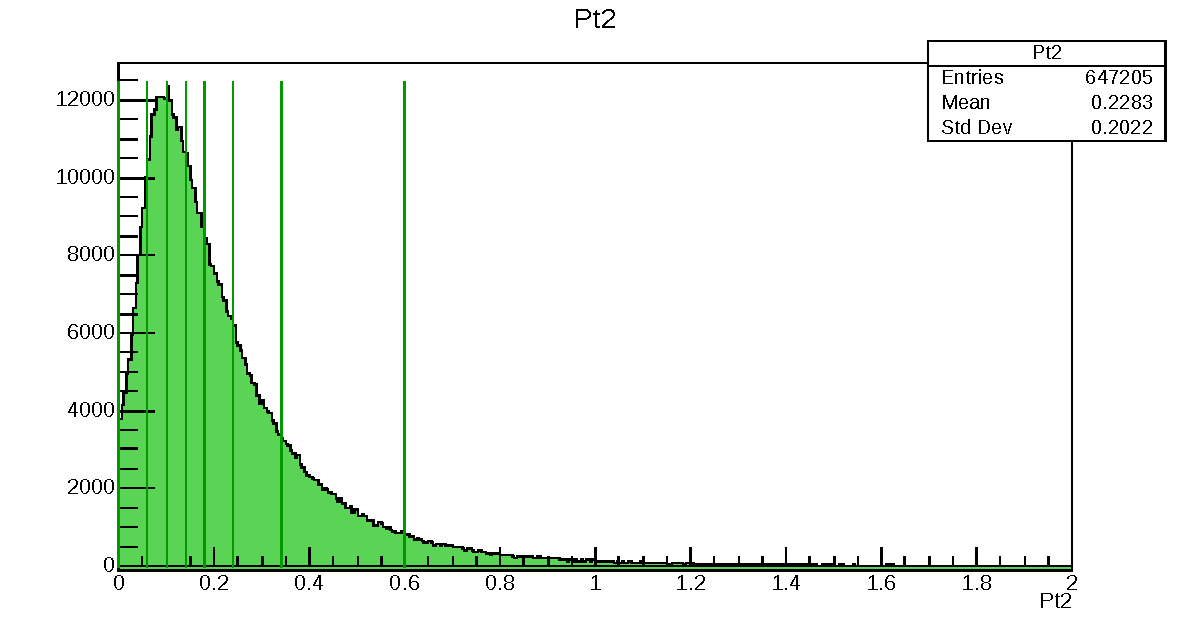
\includegraphics[width=\linewidth]{13dataanalysis/img/40_accbins_pt2.pdf}
    %         % \caption{$P_T^2$ bins.}
    %         \label{fig::acc_corr_bins_pt2}
    %     \end{subfigure}
    %     \begin{subfigure}{.5\textwidth}
    %         \centering
    %         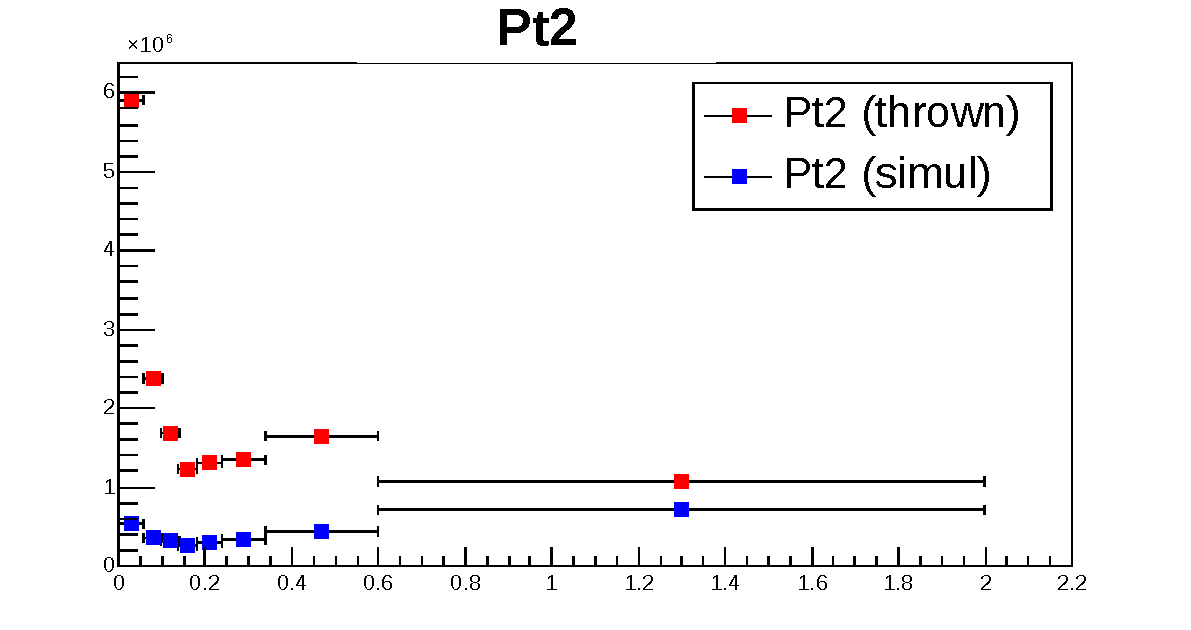
\includegraphics[width=\linewidth]{13dataanalysis/img/40_acccorr_pt2.pdf}
    %         % \caption{$P_T^2$ acceptance correction results.}
    %         \label{fig::acc_corr_pt2}
    %     \end{subfigure}
    %
    %     % phi_PQ.
    %     \begin{subfigure}{.5\textwidth}
    %         \centering
    %         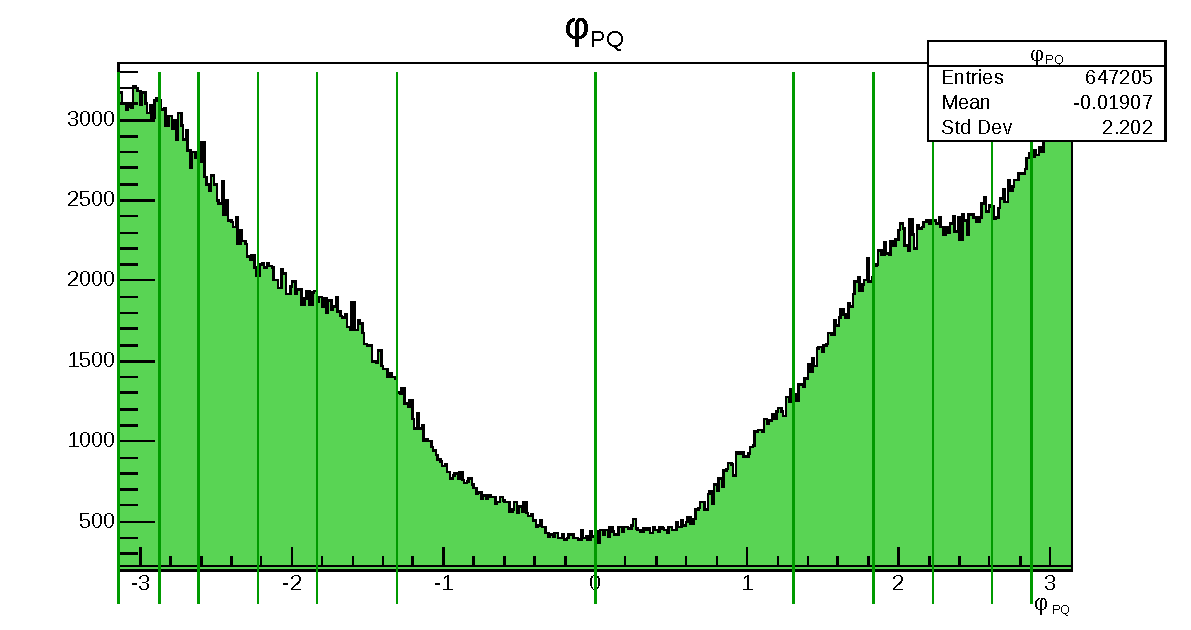
\includegraphics[width=\linewidth]{13dataanalysis/img/40_accbins_phipq.pdf}
    %         % \caption{$\phi_{PQ}$ bins.}
    %         \label{fig::acc_corr_bins_phipq}
    %     \end{subfigure}
    %     \begin{subfigure}{.5\textwidth}
    %         \centering
    %         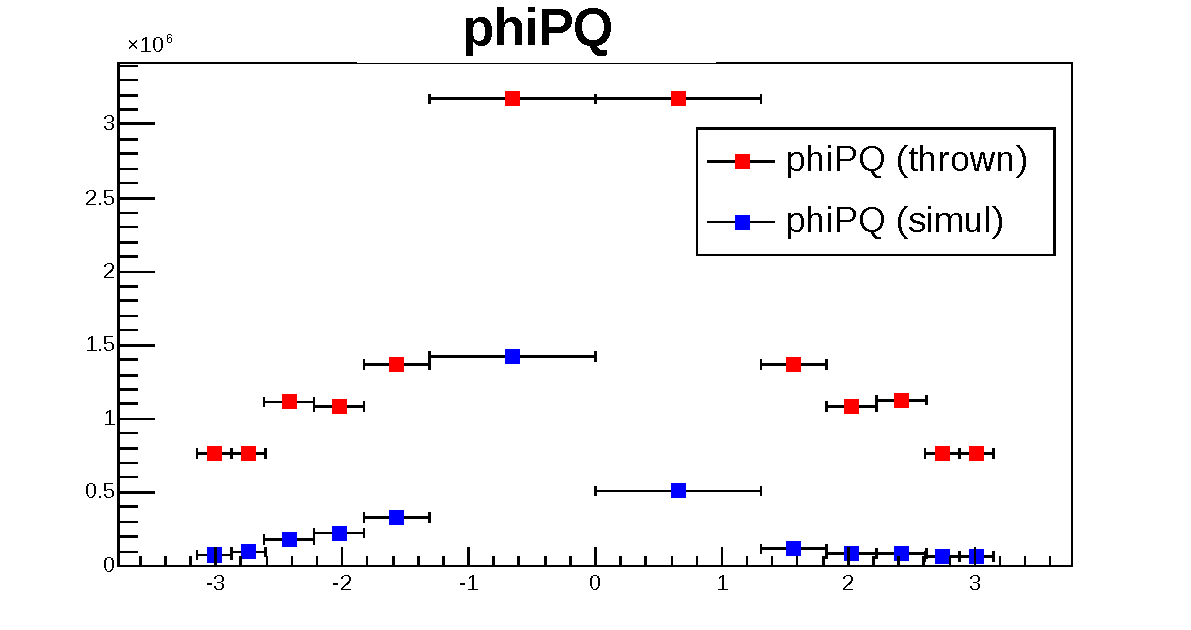
\includegraphics[width=\linewidth]{13dataanalysis/img/40_acccorr_phipq.pdf}
    %         % \caption{$\phi_{PQ}$ acceptance correction results.}
    %         \label{fig::acc_corr_phipq}
    %     \end{subfigure}
    %
    %     \caption[Acceptance correction results.]{Acceptance correction results for the kinematical variables $Q^2$, $\nu$, $z_h$, $p_T^2$, and $\phi_{PQ}$. On the left plots, the acceptance correction bin edges are shown. On the right, the number of thrown (in red) and simulated (in blue) entries for each of the variables is shown. All other variables are integrated for each plot.}
    %     \label{fig::acc_corr}
    % \end{figure}
